A general AI for games is difficult to build. This difficulty stems from the fact that game AIs have different requirements, from very tight performance constraints, to the ability to deal with rapidly changing situations, and even to the need of looking smart and challenging while at the same time being beatable by the player. 

Current technology is such that most non-playing characters are little more than "animated wallflowers", with the inability to autonomously engage the player or achieve their own goals.

We believe that there is now the opportunity to create simulations of realistic agents showing complex and unpredictable (though always reasonable) behaviors through Goal Oriented Action Planning. We believe GOAP to be a general-purpose technique that enables agents that, while being smart enough to deal with in-game situations in unpredictable ways, can still be controlled by setting their goals as the designer wishes.

In the remainder of the appendix we show how we have used Goal Oriented Action Planning (GOAP) \cite{APPENDIX_C_GOAP_BOOK} to create agents that exhibit rational-looking planning. GOAP is a planning architecture designed for controlling autonomous characters in games, originally used in games for F.E.A.R. by Monolith Productions \cite{APPENDIX_C_GOAP_FEAR} but coming from the even older work STRIPS \cite{APPENDIX_C_STRIPS}. 

GOAP presents some important challenges when applied to more than a very small set of actions to be planned, given the combinatorial explosion of the search space of the main algorithm. Our main contribution is to show how the use of a layered system of GOAP planners (which we have aptly named LGOAP) can give rise to coherent plans that span long periods of game time, and which effectively plan dozens of actions for reaching the final goal. We also discuss how modifications can be added to this basic LGOAP in order to enable agents to learn from their environment, deal with incorrect assumptions, refine subsequent planning sessions and enable the emergence (and active planning) of cooperative behaviors.


\section{Activities}
\label{sec:activities}

The virtual world contains a series of objects. Objects are the backbone of the simulation, since they define the set of available actions for a user. An object is defined as a location, its available activities, and the agents that are using it at the moment.

The location of the object is, of course, where it is (at the moment: some objects may move, such as trains, bikes, groceries, etc.). The activities of an object are a series of actions that may be performed by an agent. For example, if a certain workplace only opens between 08:00 and 17:00 for its workers, but cleaners may clean it in the evening, then we may have the following activities:

\begin{lstlisting}
{ (work,(mon,08:00,9h),(tue,08:00,9h),...)
  (clean,(mon,18:00,2h),(tue,18:00,2h),...) }
\end{lstlisting}

Activities have preconditions and consequences. Preconditions are defined as a series of predicates that must be verified in order to perform the action; the agent will have to build plans such that each precondition is met before performing the desired action. Preconditions may be about the agent statistics, location, or certificates. Example preconditions for performing the work action at the office may be:

\begin{lstlisting}
health is good; works at office; is at office
\end{lstlisting}

Post-conditions represent changes to the agent statistics or certificates. For example, the work activity may leave the agent with more money, but also more stressed, hungry, and tired:

\begin{lstlisting}
money := money + 100,stress := stress + 0.1,
hunger := hunger - 0.2,sleep := sleep - 0.1
\end{lstlisting}


\section{Agent stats}
\label{sec:agent_stats}

An agent is modeled after the traditional BDI paradigm of beliefs, desires, and intentions \cite{APPENDIX_C_BDI}. The \textit{beliefs} of an agent mirror the agent's understanding of the consequences of an action, particularly with regard to expected costs and benefits. Scenarios that require learning can be built such that the agent plans are non-optimal because of wrong beliefs. An agent \textit{desires} to maximize his happiness and well-being, while minimizing the costs associated with doing so. Happiness is defined by the system designer, and can include anything ranging from prolonged survival, to performing certain actions, or reaching a goal. The agent's \textit{intentions} are represented by his planned sequence of future actions. Intentions may be dynamically adapted and revised in order to react to a changing scenarios.

In this section we mostly discuss the desires of the agent as represented by a series of internal statistics. Beliefs are discussed in Section \ref{sec:learning}, since beliefs are represented by the agent's learned responses of the environment. Intentions are discussed in Section \ref{sec:naive_goap}, since planning and then executing one's plan is the very definition of having intentions.

Formally, an agent is defined as a location, statistics, and certificates:

\begin{lstlisting}
<agent> ::= <location>,<stats>,<certs>
\end{lstlisting}

Location simply defines where the character is located in the virtual world, that is his current \texttt{x} and \texttt{y} coordinates. Statistics define a series of internal values that change as the character performs actions, and which represent a continuous description of the general status of the agent. A statistic is defined as a value, a series of thresholds, and a series of responses. The value is simply a number between 0 and 1 that represents for example how hungry the character is, with 0 meaning starved and 1 meaning full. Agents are not all the same, and have different thresholds of attention for each statistic, and also different costs and benefits obtained from performing certain activities. Thresholds are used to transform the continuous value of statistics into discrete predicates which are then used by the planner. For example, a user who gets hungry easily may define his thresholds to hunger as:

\begin{lstlisting}
{ 95% $\rightarrow$ good; 50% $\rightarrow$ ok; 25% $\rightarrow$ bad }
\end{lstlisting}

Responses represent how much more (or less) than the agents' standard responses an agent obtains benefits or incurs penalties when performing an activity. For example, an agent who dislikes working in general but who likes working as a teacher could have responses for the \texttt{stress} statistic such as:

\begin{lstlisting}
{ work $\rightarrow$ 200%; work.teach $\rightarrow$ 25% }
\end{lstlisting}

The above means that if the agent is merely performing some work, then he will suffer twice the stress of a regular character, but if he teaches then his stress will go as low as one-quarter of the default amount. Of course having a stress statistic and a work activity is just an example, since stats and activities are highly dependent on the simulation. 

Responses and thresholds may radically change how an agent plans. Plans will always be correct, in that if a plan exists such that it allows the agent to reach the goal then the planner will find it; the planner though will first explore those plans that are "liked" by the agent, and so thresholds and responses may change the solution found.

Finally, certificates are a series of tokens that represent ownership of virtual objects, such as weapons, a home, money, etc. Some activities require that the agent owns the appropriate certificate in order to be performed, and the planner will have to take care of planning the actions to obtain a given certificate before performing the actions that require it. For example, eating may require the ownership of food, working may require having a job, traveling to a distant star-system may require knowledge of the right warp coordinates, and so on.

Agents represent their social relationships as a series of additional statistics, one for every other agent to model a relationship with; an agent may also have certificates that represent special relationships such as \texttt{married to}, \texttt{boss of}, and so on which define discrete modifiers for certain social interactions.


\section{Naïve GOAP}
\label{sec:naive_goap}

We start with a description of the naïve version of the GOAP algorithm. The algorithm requires only a queue of partially explored action plans that are expanded by adding available actions to them until a plan that satisfies the original goals is found. An action is only added to the working queue when the previous actions in the queue verify its preconditions. Satisfactory plans are then added to the solutions queue, which is then used to extract the best plan at the end of the algorithm. The algorithm in pseudo-ML could be described as:

\begin{lstlisting}
compute_best_plan() =
  Q = [a | a <- empty_plan.next_available_actions()]
  S = []
  while Q <> [] do
    plan = Q.dequeue()
    if plan.satisfies_goal() then
      S.add plan
    else
      for a in plan.next_available_actions() do
        Q.enqueue(a::plan)
  if S = [] then
    return null
  else
    return S.dequeue()
\end{lstlisting}

The queue \texttt{S} stores solutions in decreasing order according to a metric that represents the (expected) distance from the final goals. If the actions monotonically decrease the distance from the goals, then we can sort solutions in \texttt{Q} according to distance from the goals, and the algorithm can simply return the first solution it encounters:

\begin{lstlisting}
compute_best_plan() =
  Q = [a | a <- empty_plan.next_available_actions()]
  while Q <> [] do
    plan = Q.dequeue()
    if plan.satisfies_goal() then
      return plan
    else
      for a in plan.next_available_actions() do
        Q.enqueue(a::plan)
  return null
\end{lstlisting}

In our case though, we do not have a definite goal except the maximization of stats. This means that a reasonable metric could simply be the cost-to-benefit ratio:

\begin{lstlisting}
plan.value() =
  benefit = mul [a.benefit() | a <- plan]
  cost    = mul [a.cost() | a <- plan]
  benefit / cost
\end{lstlisting}

The benefit of an action is computed as the weighted sum of all the stats that increase as a consequence of that action, while the cost is computed as the weighted sum of all the stats that decrease times the duration of the action. Notice that instead of multiplying costs and benefits, which would yield approximation errors, we use a log-sum to increase numerical precision.


\section{Heuristic pruning}
\label{sec:heuristic_pruning}

The complexity of the algorithm as described above is very high; if we have a maximum number $N$ of actions that we are planning for, or if we know that there is a satisfactory plan of $N$ actions, the complexity is $O(N^k)$ where $k$ is the number of available actions at each step. Planning for the long term may require dozens or even hundreds of actions, and the resulting search space would simply be too big to be explored in real-time.

Just like human beings do not consider absurd plans, though, plans that only accumulate actions with very high costs and no benefits at all after many actions do not really need to be considered. For this reason, before adding a new plan into the queue we check if it is reasonable according to a heuristic that removes plans that are either deadly or which have an excessive cost. Deadly plans are defined as those plans that take one or more statistics below the death threshold, for example because of starvation. Excessively costly plans are defined as those that take more than a certain number of actions \texttt{M} (to avoid pruning too early) and which value is smaller than a minimum value $\epsilon$:

\begin{lstlisting}
plan.reasonable() =
  cost    = mul [a.cost() | a <- plan]
  return not_dead(self.stats + cost) && 
        (plan.length <= M || plan.value() > $\epsilon$)
\end{lstlisting}

This way even though we risk pruning some plans that incur too many costs in the beginning, we greatly reduce the size of the plan space by removing plans that feature only travel or pointlessly long repetitions of costly actions. Also, we may explicitly prune plans that "run in circles", that is we may add a boredom stat to agents such that agents refuse to consider plans that require very long sequences of "uninteresting" actions. This trims loops and other useless plans on which the planner would waste a lot of exploration effort.


\section{Acting out plans}
\label{sec:enacting_plans}

After planning, we define how a character follows his plan. A plan is a sequence of actions, where each action has certain requirements. During planning we assumed the consequences of our actions to be predictable, so that we could put the actions in the right sequence to unlock the requirements for desirable future actions with past actions. Unfortunately planning cannot foresee perfectly what the responses of the world will be (unless the simulation is completely deterministic and there are no other agents), and so the same conditions that must be verified for planning are verified before (and in some cases during) the execution of every action. When an action preconditions are not met, then the planner is run again in order to create a new plan that takes into account the unexpected situation. Also, by storing the expected costs and benefits (or a likely range of values) of each action in the plan then we can compare this estimate with the actual results; when the actual results are outside the expected values, both too bad and too good, we trigger a new planning phase to avoid acting out plans that were too optimistic, and thus may lead to bad consequences, or too pessimistic and thus wasteful.


\section{Layered GOAP}
\label{sec:layered_goap}

The goals of our agents are long-term. To give our characters the ability to correctly plan for the long term we must be able to reduce the search space far more than what can be done with simple heuristics: the longer the plans, the harder it gets to efficiently find plans or (perhaps as importantly) to stop searching when no adequate plan is found. Moreover, aggressive pruning often forces the agent into local minima. To address the problem, we have built a framework that combines multiple layers of GOAP, which we have christened LGOAP (Layered GOAP); each layer restricts the search space for successive layers, but plans at a lower granularity. The system may use as many higher-level layers for planning up to (virtual) months or years ahead as needed. Each layer creates a plan roughly of the same size as more precise layers, but it covers a different time span. The last layer plans precise actions in detail, but only for a very short time-span (it may be a few hours in a simulation, or it may be a few minutes in a game where the scenario changes in real-time very quickly such as a fighting game or a shooter). Similar hierarchical approaches have been seen in computer graphics \cite{APPENDIX_C_CLIPMAPS}, path-finding \cite{APPENDIX_C_HIERARCHICAL_PATHFINDING}, and even AI itself \cite{APPENDIX_C_HIERARCHICAL_AI}.

This means that the full planner is defined as a series of layers. The first layer plans for the longest span of time, while successive layers recursively refine its plan until finally then $n$-th layer (the last one) finds the concrete plan. Each layer contains an instance of the GOAP algorithm and a time-span for which to build the plan. Layers successive to the first also have a series of constraints that come from the previous layer(s); constraints are a pair in the form of an overall goal for the plan, and a series of allowed action-sets to which the search is restricted for the various time slots. A goal is simply a series of weights that are used to compute the benefit and the cost of an action. An example four-layered architecture is shown in Figure \ref{fig:layers}; the first layer compute the steps until the final goal, but each step cannot be acted out directly and requires more planning; the second and third layers computes the steps that cover only part of the overall plan, but these steps are more specific and realize multiple steps of the overall plan; the final layer computes the actual sequence of actions that the agent performs, but these actions only cover a short time span. Fortunately, the short time span of the concrete planner are coherent with the overall plan thanks to the layered system.

\begin{figure}
\begin{center}
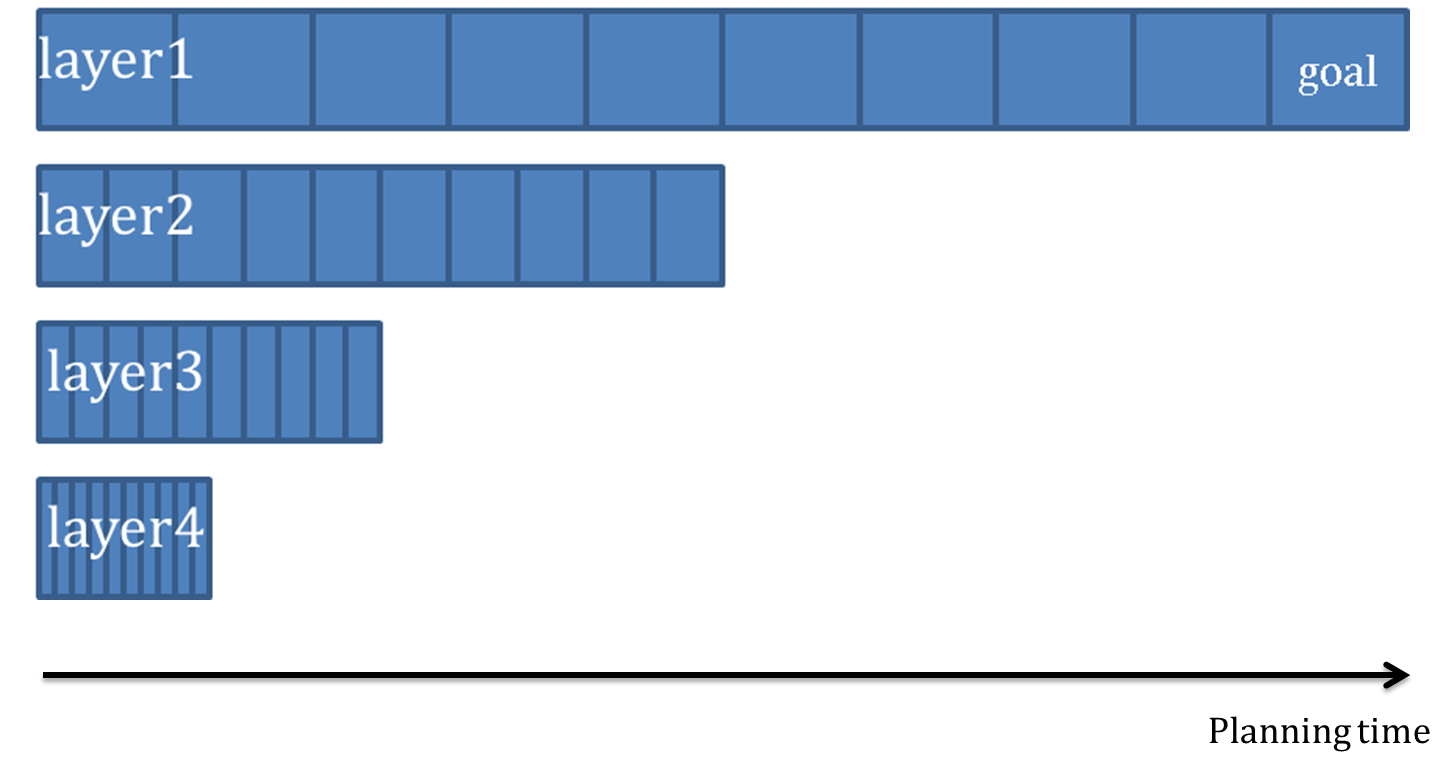
\includegraphics[scale=0.3]{Pics/layers.png}
\end{center}
\caption{Four layers planner}
\label{fig:layers}
\end{figure}  

Higher layers thus do not plan in detail; they simply plan a series of requirements that successive layers must take into account when performing their planning. Requirements steer the planning by modifying the weight of certain statistics, in order to make the planner more aware of certain statistics that change. For example, if the weights from a previous planner are:

\begin{lstlisting}
<money=0>,<food=0.1>,<stress=3.0>
\end{lstlisting}

Then an action plan that makes the character spend a lot of money but decrease his stress level a lot will be perfectly acceptable, since the higher-level planner has instructed successive layers to ignore the costs associated with decreasing the amount of money. We can refine our model further by specifying two different weights, one for the benefits and one for the costs.

This way we are still accepting plans that increase money or reduce hunger, but if we get a chance to decrease stress at the expense of either hunger or money then the plan will have a very high score. Weights are determined because the actions that the higher-level planner decides for can yield a wide range of benefits, but the planner will decide exactly what benefits are relevant and which actions are allowed only because they may be needed by the lower-level planners to create a working plan.

Higher-level planners also have the chance to restrict the set of available actions for successive plans. This restriction states the sets of allowed actions for each time slot, so that successive planners will have to restrict their search to combinations of these actions. For example it may be reasonable to have the following block of actions:

\begin{lstlisting}
walk,take-bus,drive,take-train,work,eat,chat
\end{lstlisting}

The lower-level planner can then combine them in a sequence where the user walks to the bus station, then takes the bus, then walks to work, then does his workday, and then leaves work:

\begin{lstlisting}
walk,take-bus,walk,work,chat,work,eat,
work,chat,work,walk,take-bus,walk
\end{lstlisting}

All these restrictions are actions that are designed by hand for the appropriate layer. When a planner cannot find a working plan that supports the requirements of the higher-level plan, then the higher-level layer re-plans by taking into account the new situation it has to plan from.


\section{Learning Expected Costs and Benefits}
\label{sec:learning}

The simulation is intended to be partially unpredictable, in order to provide unexpected situations to the agents. For example, the \texttt{take-train} activity may have probabilistic pre-conditions that represent the fact that the train may be late; also, the train may not take any more passengers if more than 100 people have boarded it already. The pre-conditions for taking the train may then be:

\begin{lstlisting}
money > 10,p > 0.99, passengers < 100
\end{lstlisting}

Surprises then \textit{emerge} from the simulation, for example traffic jams or trains and buses that are too full, thereby creating unpredictable situations that should be learned by the agents in order to obtain a more effective behavior.

To make agents resilient to change, we give them the ability to learn. Learning means that an agent stores a table of statistical models for actions in general, and for the same actions when performed with specific conditions (such as time or location). These statistical models store some distribution of the expected results of actions, in order to be able to better estimate the most likely range of the benefit and cost of an action for accurate planning. A very simple estimator for learning costs and benefits simply records the actual cost and benefit of an action and stores them in a rolling average and variance:

\begin{lstlisting}
avg' = $\alpha$ * x + (1.0 - $\alpha$) * avg
var' = $\alpha$ * (x - avg) * (x - avg') + (1.0 - $\alpha$) * var
\end{lstlisting}

More complex estimators could use a wealth of traditional statistical and machine learning techniques such as \cite{APPENDIX_C_REINFORCEMENT_LEARNING,APPENDIX_C_STATISTICAL_PATTERN_RECOGNITION}, etc.

With this new definition, agents can learn that an apparently valid action that often incurs in a penalty should be recorded as having a higher cost than expected, since it has a bigger chance of failing. For example, an agent who often arrives among the last agents to board a full train can learn that this specific train, only for him, does not yield the expected benefit. He may then plan to board a different train at a different time, or to use some other means of transportation. 

Similarly, we can define agents that model no-knowledge in terms of worst- (or best-) case scenarios, creating initial tentative plans that are then tried and refined while learning useful notions for re-planning.

The learning system means that while planning, each action yields a \textit{range} of expected results. This means that we have cost and benefit as the two ranges respectively $c_l, c_u$ for the cost and $b_l, b_u$ for the benefit. We have multiple ways to combine these ranges into a ratio: \textit{(i)} the pessimist algorithm simply takes the worst-case ratio of $\frac{b_l}{c_u}$ of the lowest benefit and the greatest cost; \textit{(ii)} the optimist algorithm takes the best-case ratio of $\frac{b_u}{c_l}$; \textit{(iii)} the average algorithm takes the average ratio of $\frac{b_{avg}}{c_{avg}}$, where $b_{avg} = \frac{b_u+b_l}{2}$ (and similarly for the cost); and \textit{(iv)} the distribution algorithm that maintains the joint distribution of costs and benefits in case we used some form of statistical learning technique, or to merge intervals in a new interval that uses \textit{(i)} and \textit{(ii)} as its bounds.


\subsection{Learning Whole Plans}
Our framework supports agents capable of forming habits by storing whole plans that they executed in the past. When a plan is built and performed, then we compare its expected benefits with the actual benefits. We discard plans that do not have a sufficiently high reliability, that is even if a plan performs great but in an unexpected way (that is within more than a $\delta$ value within the expected gains or losses) then we will not save this as a good plan; of course we still use our new knowledge as described above to steer the planner towards the actions of this plan, but the \textit{whole} plan is not considered successful. We maintain a working memory of old, successful plans with their associated resulting benefits. Before planning for a certain set of goals and limitations, we check the working memory to find the best known plan that realizes the goals and stays within the required limitations as dictated by the higher-level layers. If there is one or more plans that fill these needs, then we pick the best one and we skip the whole planning phase, otherwise we plan as usual. Since planning is done in real-time, this gives us agents that can create habits through which they get much faster planning whenever they can avoid re-thinking the same plan.

After an old plan is executed then we can compute a rolling average (or some other, more accurate estimation) of its reliability; this gives us a way to maintain the reliability of plans in a changing environments. It is important to pick a technique that does not suffer too much from the presence of a rare occurrence (which should be treated as statistical noise), but which is capable of adapting to trends in the game world events.


\subsection{Learning and Layers}
Higher-level plans need a way to specify the sets of actions allowed for a certain time block, in order to give freedom to the lower-level planners to combine these allowed actions sets into more specific sequences. The action-sets may be designed by those who build the concrete system, but doing so risks forcing the system to behave along some predefined "rails" when the action-sets are not expressive enough. If this happens, then the higher-level layers would be too much constrained, and they would not be able to reach good plans, but instead they would force the lower-level layers along their same constraints and sub-optimal strategies. Alternatively, we can let the system sort out the most useful action-sets by storing the actions that happen together most often. This amounts to an ulterior form of learning, since the agents will learn how to plan at a higher-level; moreover, this makes it possible to have characters who start by only planning for a few days at a time, but who gradually learn how to plan for a longer time-span.


\subsection{Implicit Social Interactions}
The learning system steers social interactions because as actions are performed, the learning abilities of an agent learn the \textit{social consequences} of the various actions. For example, an agent may learn that since another agent he likes is often present at work on Monday morning, then Monday mornings are learned to also give a boost to social interactions for no additional costs. This steers the planner towards going to work at that time slot even if it may be possible to do so at other times, because going to work in that time slot is also beneficial to social interactions. Social interactions may also make a character avoid performing actions in certain places and at certain times because doing so would be learned to be associated with meeting disliked agents that would then result in a cost for the social statistics.

To represent social relationships, a matrix of each pair of agents is maintained by the system. The matrix, which is sparse because many agents do not know each other, contains the relationship between two agents. The relationship between agents is an \textit{index} that goes from -1 (dislike), through 0 (neutral), to 1 (like). The relationship index is used to compute a multiplier for the social costs or benefits of an action. Characters automatically develop a social index by performing actions together and in vicinity. The initial social compatibility can be determined by a function on the agents personal attributes, which are their tolerance thresholds and their responses from their environment, or by different forms of defining an agent profile. Social compatibility may be defined as similarity or dissimilarity, and may even be defined by an initial randomization of likes and dislikes among agents.


\subsection{Explicit Social Interactions}
When characters like each other enough, that is more than a certain threshold, then they may choose to do some social activity together. The social activity is added to the higher-level planner at a slot that is compatible for both agents. Compatibility is measured as a positive weight for social interactions (that is in that slot it is desirable to have social interactions), and expected geographical distance. If the social interaction fails, then the relationship index is decreased; in case of a successful meeting, on the other hand, the relationship index is increased significantly.


\section{Assessment}
\label{sec:assessment}

To test our system, we devised a case study that offers a challenging environment for our agents. The system is still under construction and it is currently missing some important features, in particular learning and social actions. The most relevant part of our method though, layered planning, has been implemented and put to the test with satisfactory results.

In our game (depicted in Figure \ref{fig:case-study}) a pirate ship has to leave the pirate lair to raid the surrounding planets. These planets have different strengths and yield a different reward (loot). Not all planets can be reached right away: before traveling through some planets the ship needs to raid other planets that contain star charts required to reach the goal. The case to be solved is constructed in such a way that the ship will have to go back to the pirate lair to repair and upgrade as it progresses, and will have to refuel frequently at an ulterior location.

\begin{figure}
\begin{center}
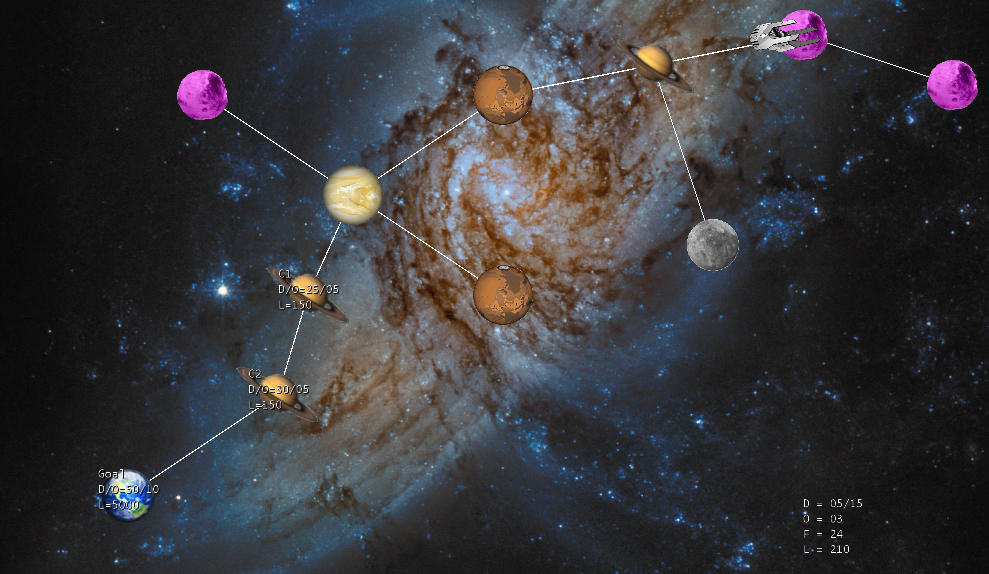
\includegraphics[scale=0.3]{Pics/Middle.png}
\end{center}
\caption{Case study}
\label{fig:case-study}
\end{figure}  

The actions available to our pirate ship are \texttt{move}, \texttt{raid}, \texttt{repair}, \texttt{upgrade}, and \texttt{refuel}. The number of actions for a plan that can reach the goal are approximately $100$, even for such a deceptively simple scenario, yielding a search space of approximately $100^5$ possible plans, given that at every step there are on average $5$ available actions that may be taken next. We have tested successfully more difficult scenarios that require even more overall actions because of the higher number of planets arranged in a much-larger grid, but we believe that the case presented here is already sufficiently challenging.

Each action has strict requirements, such as having enough fuel and the required star charts for moving to a planet, having enough loot to upgrade and so on. This still leaves many exploration options intact though, especially with regard to when to refuel, repair, and upgrade.

The current system uses two layers. The first layer plans the order in which to attack the most important planets (refueling stations and star chart owners), and the required upgrades that are needed in order to attack those planets when they are too powerful for the ship. The second layer realizes these plans to obtain these goals in the required order.

The performance of the planner is such that it is possible to perform planning in real-time. Plans are computed in less than one frame (at 60 frame per second) on a 1.8Ghz Intel Core Duo, given that plans compute few actions at a time thanks to the layering system.

The scenario offered in our case study is challenging because to reach the goal there is no single monotonically increasing stat or utility value that the ship can use to steer itself. Additionally most of the stats change in a chaotic fashion during the execution of a successful plan. Although keeping these stats high may appear desirable (for example health, fuel and loot) sometimes these must be sacrificed for long periods of time in order to reach well-defended, distant planets.
  
\begin{figure}
\begin{center}
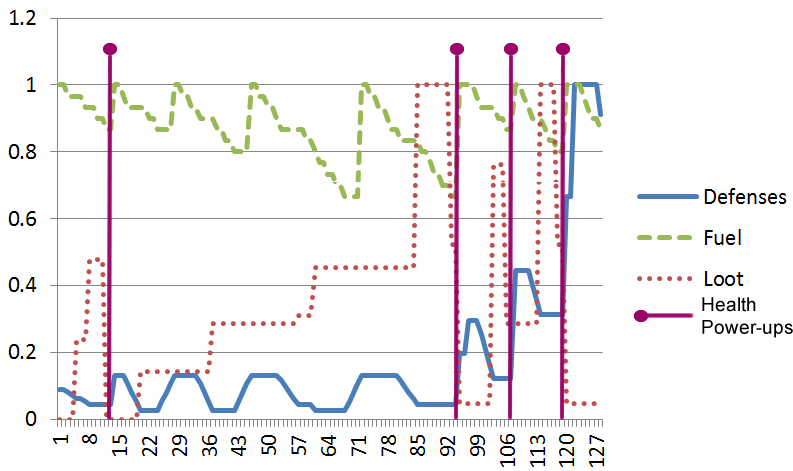
\includegraphics[scale=0.3]{Pics/graph1-stats.png}
\end{center}
\caption{Ship stats}
\label{fig:graph1-stats}
\end{figure}  

In Figure \ref{fig:graph1-stats}, it is possible to see the graph of the different stats associated with the spaceship during the simulation. The health ("Defenses") and fuel stats are continuously sacrificed to reach planets and do battle; defenses also gradually increase as the pirate ship performs upgrades ("Health power-ups"), as evidenced with the dotted vertical lines. Loot is accumulated but also spent in order to buy power ups. The first and third power ups are single, while the second and fourth are double and thus yield an even stronger increase in statistics.

\begin{figure}
\begin{center}
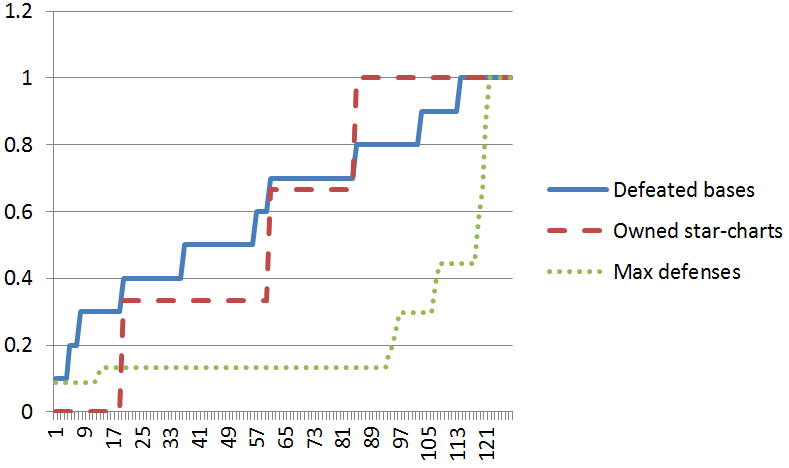
\includegraphics[scale=0.3]{Pics/graph2-goals.png}
\end{center}
\caption{Ship goals}
\label{fig:graph2-goals}
\end{figure}  
  
In Figure \ref{fig:graph2-goals}, it is possible to see the global goals, as achieved by the higher-level layer. This layer is the one responsible for planning long-term actions, and in fact we can see that the number of defeated bases, the number of owned star charts, and the defensive abilities of the ship are increased monotonically. Most notably, the success in achieving global goals is quite slow, and many actions could easily but wrongly be classified as useless by other AI systems since they do not yield a visible global advantages but they yield significant immediate disadvantages.

Finally, by lowering or increasing the agent thresholds we generate plans that are still valid (those that kill the ship are always rejected), but where the ship is ruthless and aggressive and accepts to remain damaged and under-fueled for long periods of time, or very conservative and repairing and refueling very often.

As a final loose note it is interesting to observe that the resulting behavioral pattern is very similar to that of a human player playing an RPG game, where the player alternates exploration/combat sessions with resting sessions at the closest town. The very same behavior automatically emerges from our system, thereby giving us added confidence in the quality of the technique, since we did not give any hints whatsoever that this was the desired result, instead letting the system deduce its usefulness.


\section{Missing and implemented}
\label{sec:discussion}

Our system will be extended with two major additions that we were unable to implement in time for this work: learning and adaptive planning and social interactions between agents. Learning would equip our agents with the ability to adjust their planning by including feedback from the execution of earlier plans, thereby creating an adaptive planning system able to deal with incomplete knowledge. Layers themselves could be learned, for example by finding common sequences of actions that occur often in lower-level layers that can then be grouped and considered a single action. Social interactions would make it possible for our agents to plan actions to perform together when it is advantageous to do so. Such interactions could also include coordinating group actions such as team fighting. Such a social framework could also make use of a layering system for handling groups of agents that must each behave reasonably but in a coordinated fashion. Additionally the ability to mix this planner with more traditional control structures for AIs, such as decision trees, neural networks, finite state machines, etc. would make it possible to have agents capable of more convincing local reactions to unexpected situations, such as a "fight-or-flight" reflex that does not leave the agent vulnerable to immediate dangers while planning for a full response.

Last bu not least, as soon as the planner reaches a definitive shape it will be added to Casanova in the form of a library, an extension to the language, or both.
